\documentclass[12pt, titlepage]{article}

\usepackage{booktabs}
\usepackage{tabularx}
\usepackage{hyperref}
\usepackage{graphicx} % used to import pictures
\usepackage{hyperref}
\usepackage[normalem]{ulem}
\hypersetup{
    colorlinks,
    citecolor=black,
    filecolor=black,
    linkcolor=red,
    urlcolor=blue
}
\usepackage[round]{natbib}

\title{SE 3XA3: Software Requirements Specification\\Synergy Inventory Management System (SIMS)}

\author{Team \#33, 'Sick Ideas'
		\\ Nathan Coit - 400022342
		\\ Lucas Shanks - 400029943
		\\ Cameron Van Ravens - 400020215
}

\date{\today}

%\input{../Comments}

\begin{document}

\maketitle

\pagenumbering{roman}
\tableofcontents
\listoftables
\listoffigures

\begin{table}[bp]
\caption{\bf Revision History}
\begin{tabularx}{\textwidth}{p{3cm}p{2cm}X}
\toprule {\bf Date} & {\bf Version} & {\bf Notes}\\
\midrule
Oct. 6th, 2017 & 0.0 & Initial Revision\\
Dec. 4th, 2017 & 1.0 & Revision 1\\
\bottomrule
\end{tabularx}
\end{table}

\newpage

\pagenumbering{arabic}
\noindent
This document describes the requirements for the \textit{Synergy Inventory Management System}.
\noindent
The template for the Software Requirements Specification (SRS) is a subset of the Volere template~\citep{RobertsonAndRobertson2012}.

\section{Project Drivers}

\subsection{The Purpose of the Project}
\noindent
We want to give a simple and quick-start inventory management system to small businesses and warehouses who do not have the resources or funding to set up an expensive enterprise management system.

\subsection{The Stakeholders} % taken from problem statement
\noindent
The stakeholders this application targets are small businesses with a smaller inventory size without the financial ability to use an inventory management system meant for large companies. These would usually be businesses where the owner themselves would track inventory, thus not being a complete expert in the nuances of inventory tracking.

\subsubsection{The Client}
The client for this product is also an outside reviewer. The client wishes to see a product that demonstrates the concepts of a software engineering project consisting of proper documentation and a final demonstration of the product.
\subsubsection{The Customers}
\noindent
The intended customers are small businesses and warehouses who do not have the resources, funding or need for large scale enterprise inventory management solutions. % maybe expand on this? i think this may be good though

\subsubsection{Other Stakeholders}
% Testers, Business analysts, tech experts, system designers, domain experts, usability experts... I think thats us?
The stakeholders involved in this product are the teaching assistants whose knowledge will be needed to properly document the product. These stakeholders will have a large influence over the direction of the project and the time constraints of the deliverables for the product.
\subsection{Mandated Constraints} % double check these in regards to our requirements -- consider constraints to be non-negotiable terms, where any other solution would be unacceptable.
\noindent
Description: The product shall be hosted and maintained on a public IP address to allow remote access to the platform.\\
Rationale: The customers will not have the resources or infrastructure to install, host and maintain the platform themselves.\\
Fit criterion: The site and database must be hosted remotely and always accessible by the customer.\\

% this one is sketchy...
\noindent
Description: The product shall be made using NodeJS and store data on a PostgreSQL database.\\
Rationale: The technologies used must have extensive support and must be a modern "Industry Standard".\\
Fit criterion: The product shall pass testing for the technologies and must connect to a PostgreSQL server.\\

% should be able to pull more constraints from the requirements shell
\noindent
Description: The product shall be interfaced with using HTML, CSS, and Javascript through a web browser.\\
Rationale: HTML, CSS, and javascript are the industry standard for accessing web pages and are platform independent.\\
Fit criterion: The product shall maintain standards according to the world wide web consortium.\\


\subsection{Naming Conventions and Terminology}
\noindent
SIMS: Synergy Inventory Management System. The name of the product abbreviated for ease of communication.\\
Node: NodeJS. The technology being used in the development of the product. "Node" is not used to refer to a singularity, point or vertex.\\
CSV: Comma Separated Values. CSV refers to the file type, commonly available on most systems.\\
Properly Formatted: Format matching developer's specification.\\
HTML: Hyper Text Markup Language\\
CSS: Cascading Style Sheets\\

\subsection{Relevant Facts and Assumptions}
% User characteristics should go under assumptions.
\subsubsection*{Facts}
% put facts here
% i.e. The existing enterprise software costs a lot of money
The existing application consists of 3000 lines of PHP code.\\
20 percent of all inventory items represent 80 percent of inventory costs.\\


\subsubsection*{Assumptions}
% read the volere template examples for what types of things should go here
The server hosting the web service shall be maintained by a third party web server hosting company. \\
\section{Functional Requirements}

\subsection{The Scope of the Work and the Product}
%clearly define boundaries for study of the work and requirements%
Specific tasks can be found in the Gantt chart.
Usable resources include access to a server to host the website and any open source code.
\newpage
\subsubsection{The Context of the Work}
%insert diagram
\begin{figure}[h]
    \centering
    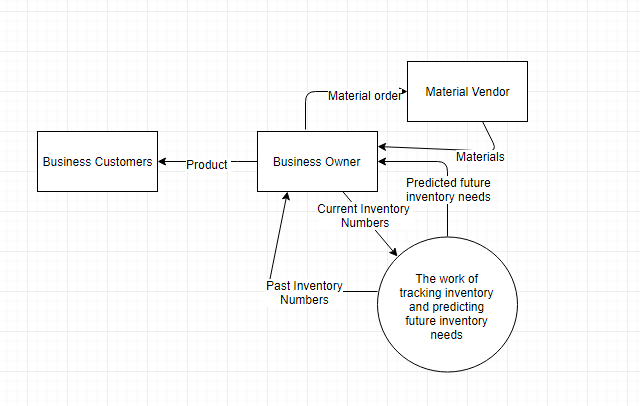
\includegraphics[scale = 1]{./img/ContextDiagram.jpg}
    \caption{Context Diagram}
    \label{fig:image1}
\end{figure}

%revolves around the work of managing user's current inventory and predicting future inventory costs
\newpage
\subsubsection{Work Partitioning}

\begin{figure}[h]
\centering

\begin{tabular}{| p{4cm} | p{3cm} | p{3cm} | p{5cm} |}
\hline
\textbf{Event Name} & \textbf{Input} & \textbf{Output} & \textbf{Summary}\\
\hline
1.User submits an inventory page & Inventory Information & Confirmation Message & Record the current inventory submitted by the user and save it to the database.\\ \hline

2.User requests inventory & User ID and Inventory ID & The selected inventory page & Return and display the requested inventory page in an editable page.\\ \hline

3.User requests homepage & - & The homepage & Return the homepage for the platform containing basic information about the product and sign up/login functionality.\\ \hline

4.User signs up & User information & - & Create an account for the user based on given information.\\ \hline

5.User requests user page & User login credentials & A user landing page & Return the landing page to the user\\ \hline

\sout{6.User requests prediction} & \sout{Item ID} & \sout{A calculated number} & \sout{Return a prediction for future inventory needs.}\\ \hline

7.User deletes an inventory page & Inventory ID & - & Delete an inventory page from the system. \\ \hline
 
8.User deletes account & User credentials & - & Remove all information on the user from the system.\\ \hline

9.User requests download of their inventory & User credentials and inventory ID/IDs & A csv file of inventory information & Allow the user to download a local copy of their inventory.\\ \hline


\hline
\end{tabular}

\caption{Work Partitioning}
\label{fig:table1}

\end{figure}


\subsubsection{Individual Product Use Cases}
Access management handles access control to the same inventory management system differently between the two types of user groups: admin and user. While admin accounts receive full functionality to the application, regular users shall have access restricted and must be tied to administrative accounts. User access features can be found above under work partitioning and records all events that may occur in a user session.\\

\subsection{Functional Requirements}
req\_ID: \label{REQ1}REQ1\\
Description: The application shall be accessible at a URL in most browsers.\\
Fit Criterion: The application must appear in the browser when accessing its URL.\\

\noindent
req\_ID: \label{REQ2}REQ2\\
Description: The user shall log in to grant access to the product and their data.\\
Fit Criterion: The user must not be able to access the application or their data before they have logged in.\\

\noindent
req\_ID: \label{REQ3}REQ3\\
Description: The user shall be brought to a main overview page upon logging into the application.\\
Fit Criterion: After logging in, the main overview page must be displayed.\\

\noindent
req\_ID: \label{REQ4}REQ4\\
Description: The user shall be able to add items to the database.\\
Fit Criterion: The user must be able to enter data, and have it stored on the database.\\

\noindent
req\_ID: \label{REQ5}REQ5\\
Description: The user shall be able to bulk add items to the database from information in a CSV document.\\
Fit Criterion: The user must have the option to read and store data from a CSV file that they provide to the application.\\

\noindent
req\_ID: \label{REQ6}REQ6\\
Description: The user shall be able to access and edit their data in the database.\\
Fit Criterion: The user must be able to view their stored items and edit the data correlated to them.\\

\noindent
req\_ID: \label{REQ7}REQ7\\
Description: The application shall be mobile-responsive.\\
Fit Criterion: The application must be completely usable and fluid on a smaller/mobile phone screen.\\

\noindent
req\_ID: \label{REQ8}REQ8\\
Description: The user shall be able to allow other users to access their page, with either Admin or User access levels.\\
Fit Criterion: The user must be able to add extra logins to their account, with controllable access levels.\\

\noindent
req\_ID: \label{REQ9}REQ9\\
Description: The database shall have a recent back up in case of emergency.\\
Fit Criterion: A back up of the server shall be no older than one week.\\

\section{Non-functional Requirements} %header
\subsection{Look and Feel Requirements}
This application shall have a simple yet professional style with a consistent overall layout.\\
Fit Criterion: The majority of users shall find the website visually appealing.\\

\noindent There shall be emphasis put upon rational space usage.\\
Fit Criterion: A single web page should not take more than 1 minute to navigate through.\\

\noindent Sleek design shall entice the user to be involved with the product, as well invoke feelings of trust and reliability between the user and the application over regular use.\\
Fit Criterion: A majority of first time users should use the product again in the future.

\subsection{Usability and Humanity Requirements}
The primary usability requirement is to provide the user with a clean, simple, user-friendly interface.\\
Fit Criterion: All options and fields on the web page shall not be ambiguous.\\

\noindent Information and choices shall be presented in a clear and concise manner with stress on lack of ambiguity.\\
Fit Criterion: The majority of users shall understand how to use the page upon first use.\\

\noindent All functionality shall be intuitive and be usable with no training.\\
Fit Criterion: No training shall be needed to use the product.\\

\noindent The application shall also ensure reliable functionality across mobile devices and browsers and shall support screen readers for impaired users.\\
Fit Criterion: Web page shall be accessible from mobile phones, and be readable by screen reader software.

\subsection{Performance Requirements}
The maximum server response time for all activities should be no longer than 5 seconds.\\

\subsection{Operational and Environmental Requirements}
The product shall be accessible through most popular web browsers.\\
Fit Criterion: Website accessible through Google Chrome, Mozilla Firefox, Opera, and Internet Explorer 9 and above.\\

\subsection{Maintainability and Support Requirements}
Server updates should be done overnight during low server load times.\\
Fit Criterion: server shall be down no longer than 20 minutes between the hours of 12am and 5am EST once a month.

\subsection{Security Requirements}
Only registered users can access the product by logging into their user account.\\
Users can only view their own inventory and data.\\

\subsection{Cultural Requirements}
Product shall not offend \%100 of users.

\subsection{Legal Requirements}
Personal information shall be implemented so as to comply with the Data Protection Act.\\
Fit Criterion: Lawyer's opinion that the product does not break any laws.\\

\subsection{Health and Safety Requirements}
The product shall run on environmentally friendly server spaces.\\
\section{Project Issues}
\subsection{Open Issues}
\sout{How to handle multiple users editing a single inventory at once.} Decision to only allow one user to edit a page at a time, while other can view it updates upon request. \\

\subsection{Off-the-Shelf Solutions}
One simple solution is managing inventory with paper or a manually made spreadsheet\\
Existing inventory management system Fishbowl Inventory starts at \$4,395 per user licence.\\

\subsection{New Problems}
Any users currently using an separate application or other means of managing inventory must transfer all data into their new environment.\\
Users require a personal machine with an internet connection to access inventory.\\

\subsection{Tasks}
In order to implement this project, the waterfall method is being used. This follows the phases of requirements, design, implementation, verification, maintenance. The following points illustrate the approach that will be taken to deliver the final product.\\

\noindent Proof of Concept Demo\\
Required operational date: 10/18/17\\
This demonstration includes a low-level working prototype including the primary features present in the final design including user log-in and account creation, storing and retrieving user inventory information.\\
The prototype must be responsive when requests are made to access and store information.\\

\noindent Revision 0 Demonstration\\
Required operational date: 11/15/17\\
This demonstration will include the fully tested, finished application revised with feedback from the proof of concept demo with all working events. This application should be accessible online. \\

\noindent Final Demonstration\\
Required operational date: 11/29/17\\
A working copy of the product shall be demonstrated to the client and stakeholders.\\

\noindent Revision 1\\
Required operational date: 12/5/17\\
The final revision and changes of the documentation and project shall be uploaded to the GitLab repository.\\

\subsection{Migration to the New Product}
%define csv and properly formatted
Users should be able to import a properly formatted csv file to instantiate their inventory.\\

\subsection{Risks}
The user must commit time to transfer current database information into the new database.\\
Features may not fulfill user requirements.\\
Software may provide inaccurate inventory prediction.\\
Inventories may be lost in event of server failure.\\


\subsection{Costs}
Not applicable.
%no money costs, costs of time say # of hours * functional requirements
\subsection{User Documentation and Training}
%an about page/quickstart page/downloadable user documentation/ service manual for hosting page/ our group in charge of keeping document up to date
Technical specifications to accompany the product:\\
User manual\\
About page accessible through the product\\
Documentation will be maintained by the developers.\\

\subsection{Waiting Room}
Not applicable.
%The waiting room includes requirements that will not be part of the next release but could be included in future releases of the product.%
%language support? Not applicable for rev0%

\subsection{Ideas for Solutions} %does not apply to rev0%
Not applicable. 

\bibliographystyle{plainnat}

\bibliography{SRS}

\newpage

\section{Appendix}

This section has been added to the Volere template.  This is where you can place
additional information.

\subsection{Symbolic Parameters}

The definition of the requirements will likely call for SYMBOLIC\_CONSTANTS.
Their values are defined in this section for easy maintenance.


\end{document}
